\chapter{Alternating Current}
\begin{itemize}
    \item An \emph{alternating current (a.c.) source} creates an electrical \emph{current} that varies in magnitude \emph{and} direction \emph{periodically with time}, as opposed to a \emph{direct current} (d.c.) source where the \emph{direction} of the current stays \emph{constant}. 
    \item Alternating current \emph{must change direction}. For instance, the following two functions, namely \(I=sin(t)+1\) and \(I=cos(t)+1\), are both (varying) direct currents.
    \begin{center}
        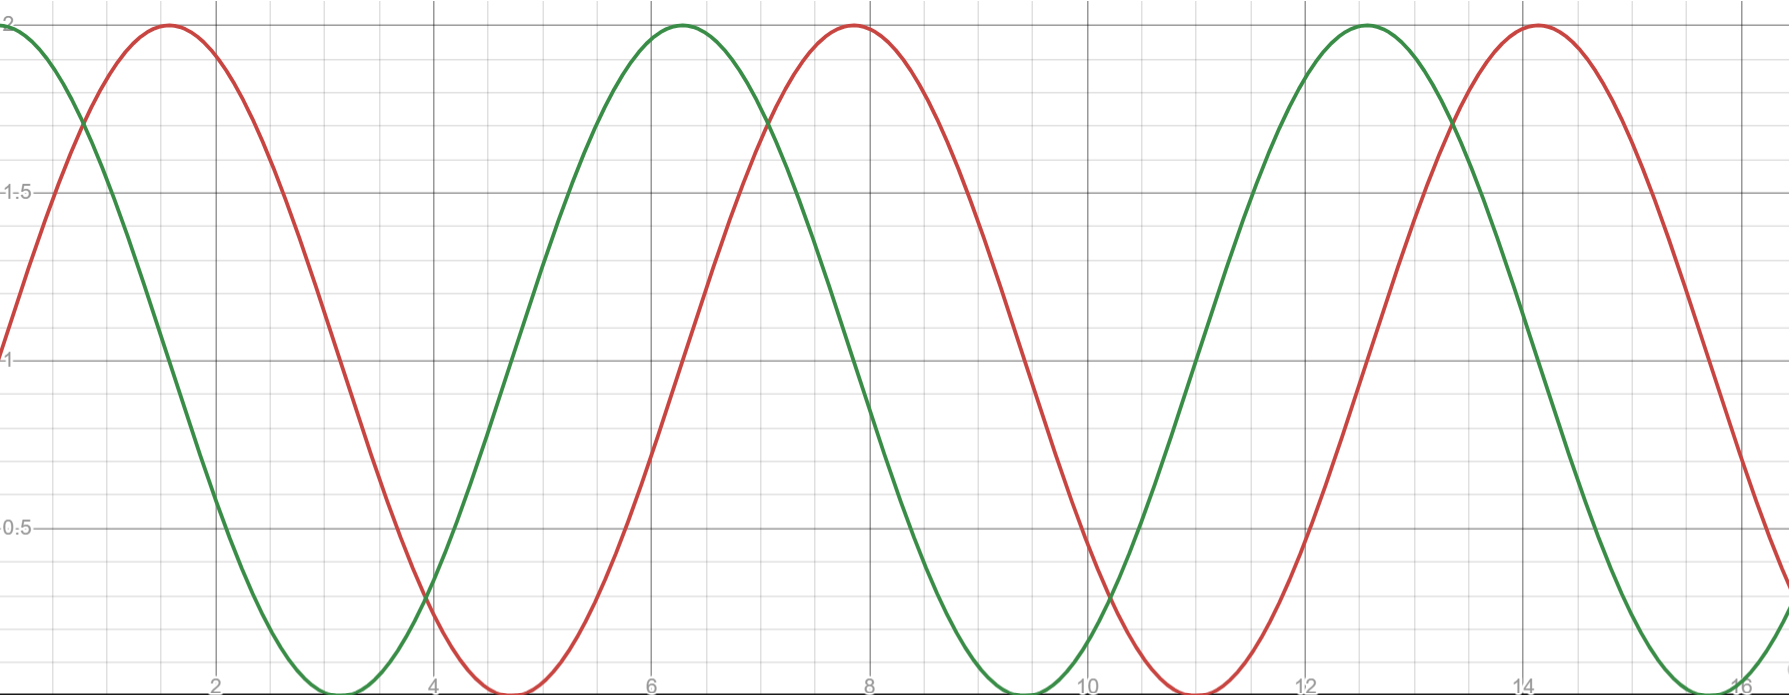
\includegraphics[width=\textwidth-25pt]{../images/Varying-Direct-Current.png}
        \captionsetup{type=figure}
        \caption[figure]{\ref{Varying direct current} Direct currents.}
    \end{center}
    \item A \(k\,\text{V}\) \(f\,\text{Hz}\) a.c. supply is one which has \(\text{V}_\text{rms}=k\) and frequency \(f\).
    \item The \emph{root-mean-square} (r.m.s.) value \(I_{\text{rms}}\) (or \(V\text{rms}\)) of an \emph{alternating current} (or alternating voltage) is the value of a \emph{steady direct current} (or direct voltage) that would produce the \emph{same average power} in a given resistor.
    \item We denote the mean value of a quantity \(x\) by \(\langle x \rangle\). So, \(x_{rms}=\sqrt{\langle x^2 \rangle}\), and it also holds that
    \[\langle P \rangle=I_\text{rms}^2R=\frac{V_\text{rms}^2}{R}.\]
    \item Steps to determine the rms value: square \(\to\) mean  \(\to\) root.
    \begin{enumerate}
        \item Square all values of \(I\) (or \(V\)).
        \item Find the mean square value \(\langle I^2 \rangle\) (or \(\langle V^2 \rangle\)). This is just the area under the graph of \(I^2\) (or \(V^2\)) against \(t\) in one period.
        \item Square root the value obtained above.
    \end{enumerate}
    \item Note that for a \emph{full wave sinusoidal} alternating current (which an be assumed unless otherwise stated), 
    \[\langle P \rangle=\frac{1}{2}P_0,\qquad V_{\text{rms}}=\frac{1}{\sqrt{2}}V_0,\quad\text{and}\quad I_{\text{rms}}=\frac{1}{\sqrt{2}}I_0.\]
    \item Explain why in the selection of a suitable fuse, the r.m.s. current is considered instead of the peak current. \hspace*{\fill} [2]
    \begin{itemize}
        \item The fuse will only be blown if its rating is \emph{lower} than the \emph{r.m.s.} current. \hspace*{\fill} [1]
        \item The peak current only occurs for a very short time. Hence, the \emph{heat dissipated} by the peak current is \emph{insufficient} to blow the fuse. \hspace*{\fill} [1]
    \end{itemize}
    \item An \emph{ideal transformer} is 100\% efficient with no power loss, such that the input and output power are equal.
    \item Let \(N_P\), \(V_P\), and \(I_P\) be the number of turns, rms voltage, and rms current, respectively, in the primary winding. (The peak voltage/current works too, for a sinusoidal wave form, by proportionality.) Similarly define \(N_S\), \(V_S\), and \(I_S\) for the secondary winding. Then, the turns ratio is defined as
    \[\frac{N_S}{N_P}=\frac{V_S}{V_P}=\frac{I_P}{I_S}.\]
    (To quickly determine which side carries a greater voltage, we can use the principle of `more turns, more voltage'.)
    \item A step up transformer is one that increases voltage, i.e. \(V_S>V_P\) (or \(N_S>N_P\)).
    \item A step down transformer is one that decreases voltage, i.e. \(V_P>V_S\) (or \(N_P>N_S\)).
    \begin{center}
        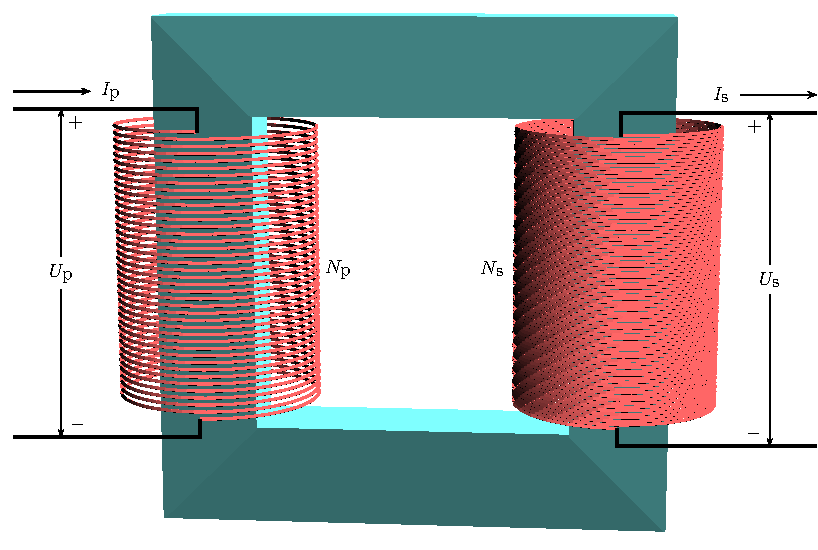
\includegraphics[width=\textwidth-30pt]{../images/Transformer/TransformerCropped.pdf}
        \captionsetup{type=figure}
        \captionof{figure}{\ref{Transformer} A step-up transformer with \(N_P=40\) and \(N_S=80\).}
    \end{center}
    \begin{center}
        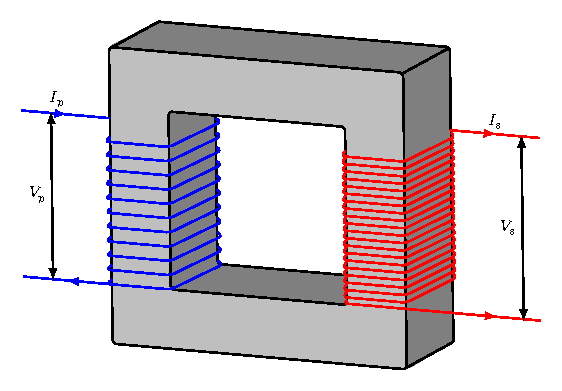
\includegraphics[width=\textwidth-30pt]{../images/Another-Transformer/Another-Transformer.pdf}
        \captionsetup{type=figure}
        \captionof{figure}{\ref{Another Transformer} Another step-up transformer.}
    \end{center}
    \item Transformers cannot be used for \emph{constant} direct current. Since there is no change in voltage/current, no emf will be (constantly) induced in the secondary coil. 
    \item When the direct current varies, however, there will be an \emph{alternating} current induced.
    \item Energy loss in a transformer.
    \begin{enumerate}
        \item Winding resistance. Current flowing through the windings causes \emph{resistive heating} of the conductors.
        \item Hysteresis losses. Each time the \emph{magnetic field is reversed}, a small amount of energy is lost due to hysteresis within the core.
        \item Magnetostriction. Magnetic flux in a ferromagnetic fore causes it to physically expand and contract slightly with each cycle of the magnetic field. This produces a \emph{buzzing sound} and can cause losses due to \emph{frictional heating}.
        \item Mechanical losses. The alternating magnetic field causes fluctuating forces between the primary and secondary windings. These cause vibrations within nearby metalwork, adding to the \emph{buzzing noise} and \emph{consuming a small amount of power}.
    \end{enumerate}
    \begin{example}{}{}
        State two reasons why soft iron, which is easily magnetised and demagnetised, is used as the core.
        \begin{itemize}
            \item Soft iron has low hysteresis losses; energy dissipated each cycle of magnetisation is reduced.
            \item Soft iron's quick magnetisation and demagnetisation allows for a high frequency alternating current.
            \item Quick magnetisation means that there are no residual effects if the transformer is not in use.
        \end{itemize}
    \end{example}
    \begin{example}{}{}
        Explain how the lamination of the core reduces energy losses.
        \begin{itemize}
            \item The changing magnetic flux linkage induces eddy currents. 
            \item The laminated sheets block the path of eddy currents, so smaller loops of eddy currents form within each laminate.
            \item Hence, thermal energy losses are reduced.
        \end{itemize}
    \end{example}
    \item Power is typically transmitted at high voltages to minimise the power lost during transmission, which is proportional to \(1/V^2\) (r.m.s.) as seen below.
    \begin{example}{}{}
        A power plant sends an average of \(\langle P \rangle\) watts of electrical power to a town by electrical cables, that have a total resistance of \(R\) ohms. What is the power lost in the cables when the power was transmitted at \(V\) volts? 
    
        \rule{20cm-137.0549pt-25pt}{0.05mm}\vspace{0.5\baselineskip}
        \begin{enumerate}
            \item[\textcolor{green!70!black}{\checkmark}] Power lost in the cables\({}=I^2R=\left(\highlight[green!70]{\dfrac{\langle P \rangle}{V}}\right)^2R\).
            \item[\textcolor{red}{\(\times\)}] Power lost in the cables\({}=V^2/R\). This is \textcolor{red}{incorrect} because \(V\) is not the voltage across the cables. Rather, it is the rms voltage of the power plant (a.c. source). 
        \end{enumerate}
    \end{example}
    \item Rectification.
    \begin{itemize}
        \item A \emph{half-wave rectification} converts only \emph{half} of the a.c. into d.c. by allowing current flow in only one direction.
        \begin{figure}[h]
            \centering
            \begin{subfigure}[c]{0.45\textwidth}
                \centering
                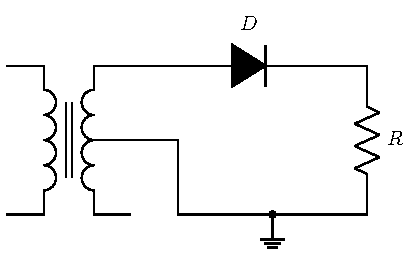
\includegraphics[width=0.7\linewidth]{../images/Half-Wave-Rectification/Half-Wave-Rectification.pdf}
                \caption{\ref{Half-Wave-Recification-Circuit} Circuit diagram.}
            \end{subfigure}%
            \begin{subfigure}[c]{0.45\textwidth}
                \centering
                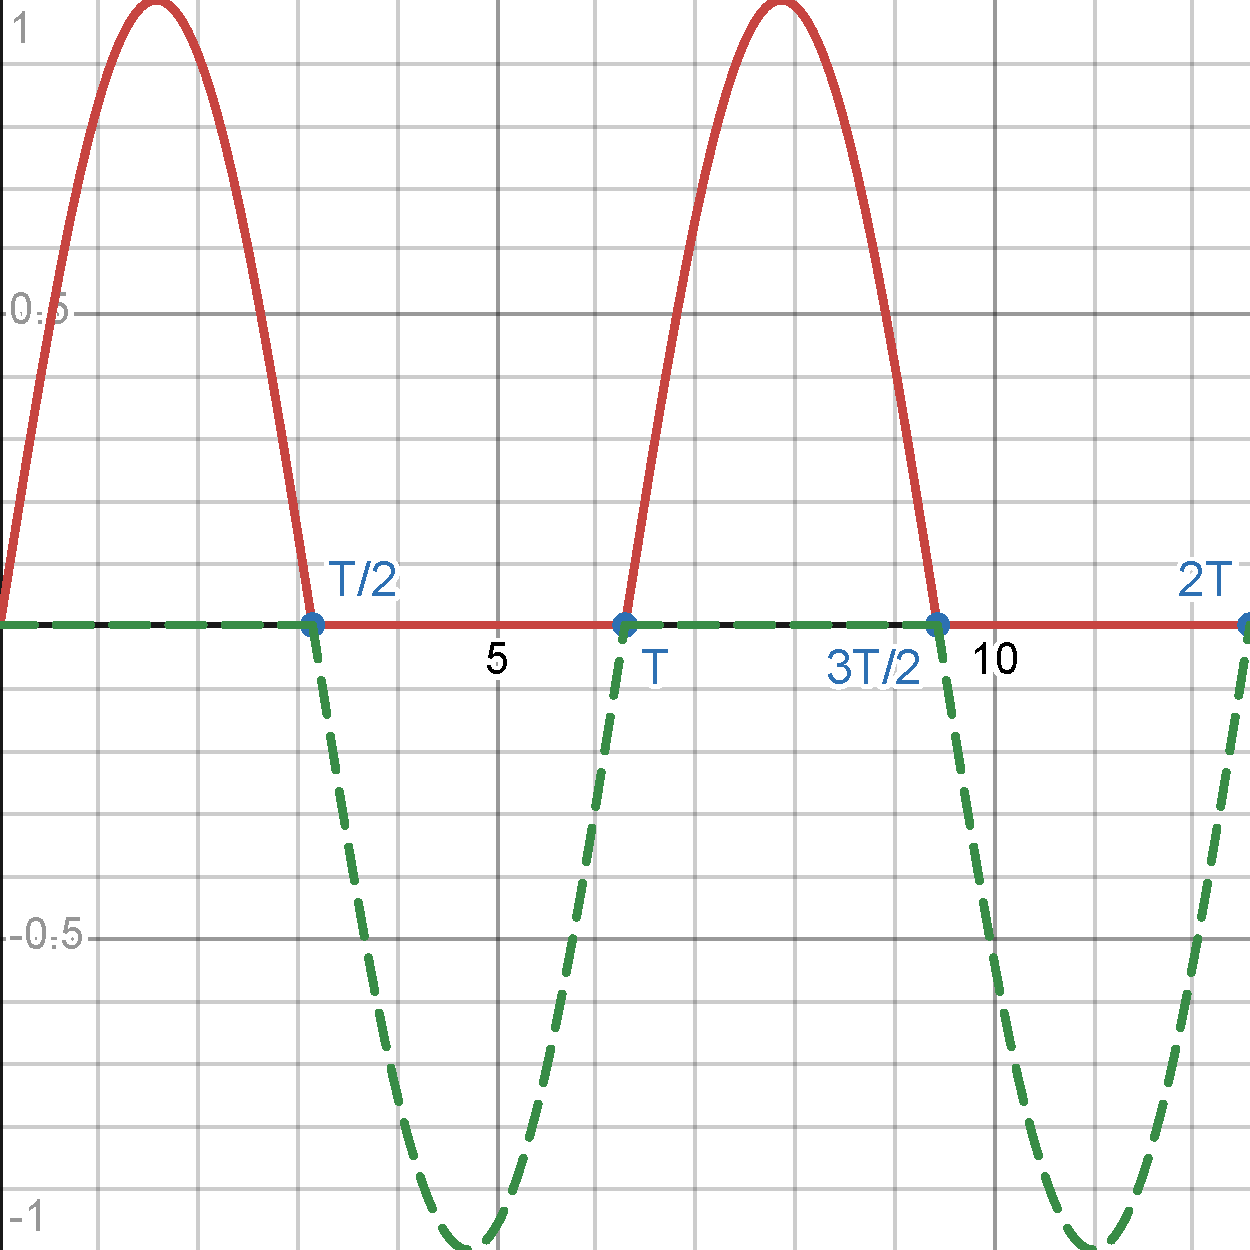
\includegraphics[width=0.7\linewidth]{../images/Half-Wave-Rectification/Half-Wave-Rectification-Graph.pdf}
                \caption{\ref{Half-Wave-Recification-Graph} The red and green lines denote the \(V_R-t\) and \(V_D-t\) graphs, respectively.}
            \end{subfigure}
            \caption{Half-wave rectification.}
        \end{figure}
        \begin{itemize}
            \item First half cycle (`positive' \(V\) and \(I\))
            \begin{itemize}
                \item The diode is \emph{forward-biased} and has almost zero resistance, allowing the flow of current through the circuit.
                \item There is negligible p.d. (approximately zero) across the diode due to the low resistance.
                \item Thus, p.d. \(V_R\) across the resistor \(R\) is equal to the a.c. input voltage.
                \item So, when the diode is forward-biased, \(V_R\) follows the a.c. supply.
            \end{itemize}
            \item Latter half cycle (`negative' \(V\) and \(I\))
            \begin{itemize}
                \item The diode is now \emph{reverse-biased} and has almost infinite resistance, such that only a negligible current flows through it.
                \item The p.d. across the diode is equal to the a.c. input supply voltage as its resistance is very much larger than \(R\).
                \item Thus, the p.d. \(V_R\) across \(R\) is negligible.
                \item So, when the diode is reverse-biased, \(V_R=0\).
            \end{itemize}
        \end{itemize}
        \item A \emph{full-wave rectification} converts \emph{all} of the a.c. into d.c. by inverting the negative current flow into positive current flow.
        \begin{figure}[h]
            \centering
            \begin{subfigure}[c]{0.45\textwidth}
                \centering
                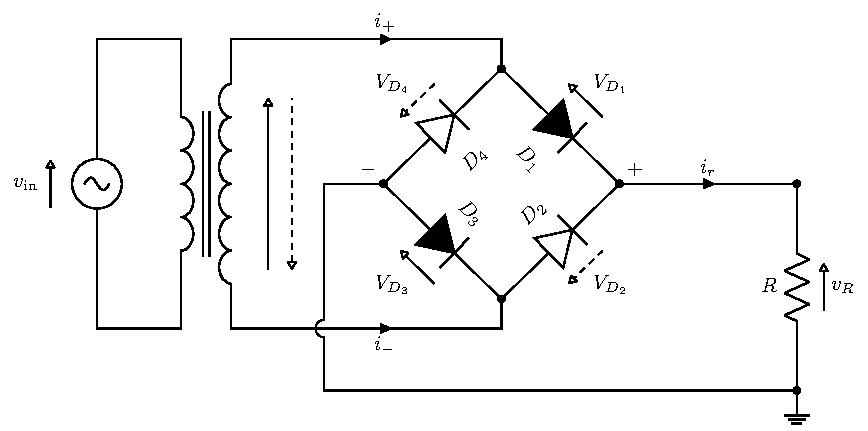
\includegraphics[width=0.7\linewidth]{../images/Full-Wave-Rectification/Full-Wave-Rectification.pdf}
                \caption{\ref{Full-Wave-Rectificaion-Circuit} Circuit diagram.}
            \end{subfigure}%
            \begin{subfigure}[c]{0.45\textwidth}
                \centering
                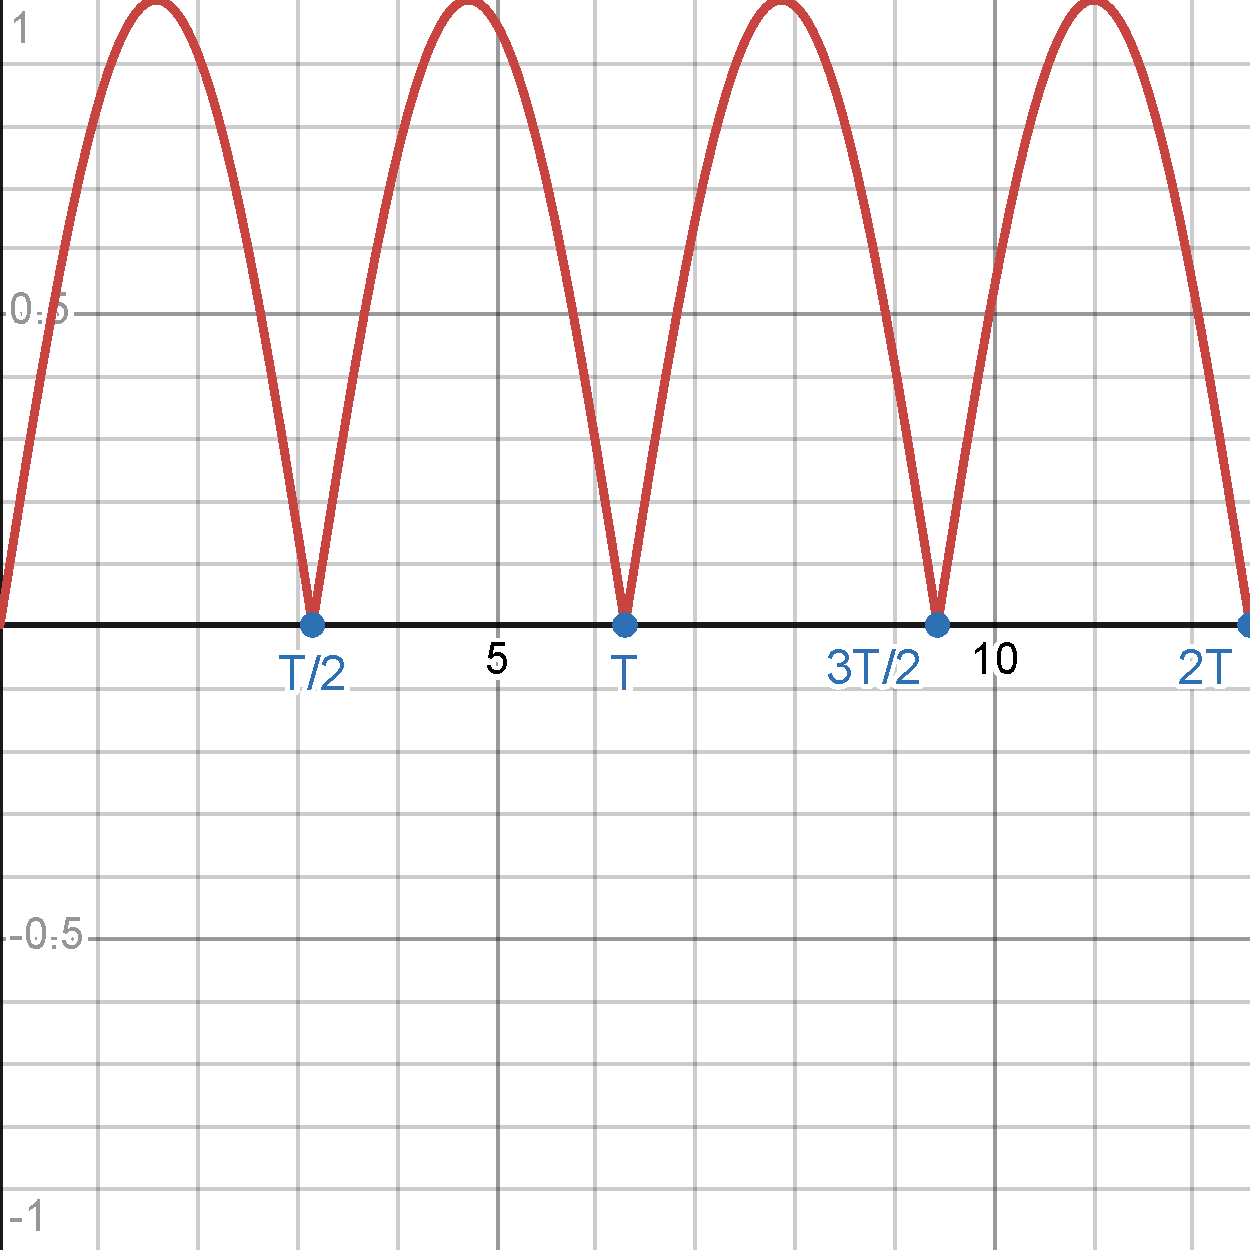
\includegraphics[width=0.7\linewidth]{../images/Full-Wave-Rectification/Full-Wave-Rectification-Graph.pdf}
                \caption{\ref{Full-Wave-Rectification-Graph} The \(V_R-t\) graph.}
            \end{subfigure}
            \caption{Full-wave rectification.}
        \end{figure} 
    \end{itemize}
\end{itemize}